\documentclass{article}

\usepackage{arxiv}

\usepackage[utf8]{inputenc} % allow utf-8 input
\usepackage[T1]{fontenc}    % use 8-bit T1 fonts
\usepackage{hyperref}       % hyperlinks
\usepackage{url}            % simple URL typesetting
\usepackage{booktabs}       % professional-quality tables
\usepackage{amsfonts}       % blackboard math symbols
\usepackage{nicefrac}       % compact symbols for 1/2, etc.
\usepackage{microtype}      % microtypography
\usepackage{lipsum}		% Can be removed after putting your text content
\usepackage{graphicx}
\usepackage[numbers]{natbib}
\usepackage{doi}
\usepackage{amsmath}

\title{Lagrange-ng: The next generation of the DEC model}

\author{\href{https://orcid.org/0000-0002-9130-6878}{\includegraphics[scale=0.06]{orcid.pdf}\hspace{1mm}Ben Bettisworth}\\
  Computational Molecular Evolution\\
  Heidelberg Institute for Theoretical Studies\\
  Heidelberg, Germany \\
  \texttt{ben.bettisworth@h-its.org} \\
  %% examples of more authors
  \And
  Alexandros Stamatakis\\
  Computational Molecular Evolution\\
  Heidelberg Institute for Theoretical Studies\\
  Heidelberg, Germany\\
  \texttt{alexandros.stamatakis@h-its.org} \\
}

\renewcommand{\shorttitle}{\textit{arXiv} Template}

%%% Add PDF metadata to help others organize their library
%%% Once the PDF is generated, you can check the metadata with
%%% $ pdfinfo template.pdf
\hypersetup{
  pdftitle={Lagrange-ng Supplemental Material},
  pdfsubject={q-bio.NC, q-bio.QM},
  pdfauthor={Ben Bettisworth, Alexandros Stamatakis},
  pdfkeywords={},
}

\begin{document}
\maketitle

\section{Background}

Computation of the likelihood of a particular set of parameters under the DEC model proceeds in a fashion similar to the
Felsenstein algorithm. In this algorithm, the computation starts from the tips and moves towards the root, storing
intermediate results in buffers called conditional likelihood vectors. Please see \cite{yang2006computational} for a
much more detailed explanation, including a detailed discussion about the savings involved with such a scheme. What is
relevant for the discussion here is that the Felsenstein algorithm avoids excess computation by noticing that, at
certain points in the computation of a likelihood on a tree, the only relevant number is the likelihood
\textit{conditioned on the current state}.

\section{Methods and Algorithms}
\label{sec:methods}

Lagrange utilizes a task based parallelization scheme in which each node of the tree is assigned as a task. In order to
compute the results for a generic node of the tree results for its two children must be computed. This involves
computing
\begin{enumerate}
  \item The right and left rate matrices: $Q_r$, $Q_l$,
  \item The right and left transition matrices: $P_r = e^{Q_r}$ and $P_l = e^{Q_l}$ respectively,
  \item The result of the Markov process along the left and right branches: $w_r = P_r v_r$ and $w_l = P_l v_l$
        respectively,
  \item The weighted combination of $w_r$ and $w_l$, $v_t$.
\end{enumerate}
Together, these operations make up a single task for a worker. However, as it can be seen above, the task can be
subdivided into smaller parts, which we will call operations. For the purposes of this paper, we will label each of the
operations as
\begin{enumerate}
  \item Make Rate Matrix Operation,
  \item Expm Operation,
  \item Dispersion Operation and,
  \item Split Operation.
\end{enumerate}
In order to more easily support computation on other platforms, such as GPUs, we have separated the operations from the
memory buffers which are required to store the intermediate result needed for likelihood computation. For example, in
Figure~\ref{fig:simple-operations} we show an unspecified node and its associated operations. In each operation, there
is a set of indices which indicate the location of the assigned memory buffer. Additionally, they store the last
execution clock point, which is discussed later.

Each operation is typically small enough that it can't justify being its own separate task. Still, if the tree
topology and branch lengths are appropriate, these operations can be shared between two tasks. For example, consider the
tree topology in Figure~\ref{fig:ultra}. Here, two of the branches share the same length, $1.0$, and so if they also
share a rate matrix, then the result of this computation will be the same. Therefore, the computation of the likelihood
of this tree can be accelerated by computing $e^Q$ only once, and saving the result.

In order to avoid re-computation of the same result, Lagrange-ng allows for the sharing of operations between tasks.
However, when computing with multiple threads, this introduces the possibility of computing with stale values from
dependant operations when performing successive evaluations of the likelihood with changed model parameters, as in most
optimization routines.

To avoid stale data, we use a clock based method to enforce a total ordering on the computation of operations. Readers
familiar with vector clocks will recognize this as a vector clock with the number of distributed elements set to one.
After the evaluation of each operation, a time is recorded in the evaluated operation, and the clock incremented. When
we wish to know if a operation is ready, all that needs to be done is to check if the clocks of its immediate dependant
operations show a larger value. If this is the case, then the dependant operations have already been evaluated, and the
operation is ready.

By carefully dividing the tasks into operations, merging identical operations between tasks, and enforcing a total order
on the computation of operations, we can implement an extremely effective task based parallelization scheme.

\begin{figure}
  \centering
  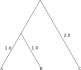
\includegraphics[width=.5\linewidth]{figures/simple-tree-ultrametric.pdf}
  \caption{A simple ultrametric tree.}
  \label{fig:ultra}
\end{figure}

\begin{figure}
  \centering
  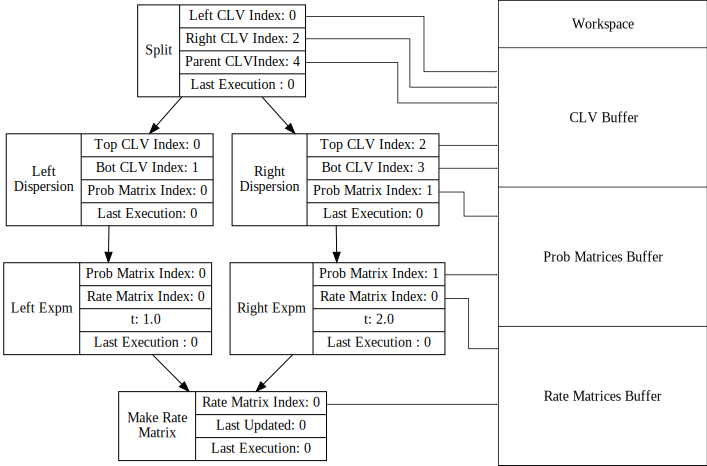
\includegraphics[width=\linewidth]{figures/simple-operations.pdf}
  \caption{An example set of operations for an generic unspecified node.}
  \label{fig:simple-operations}
\end{figure}

\begin{figure}
  \centering
  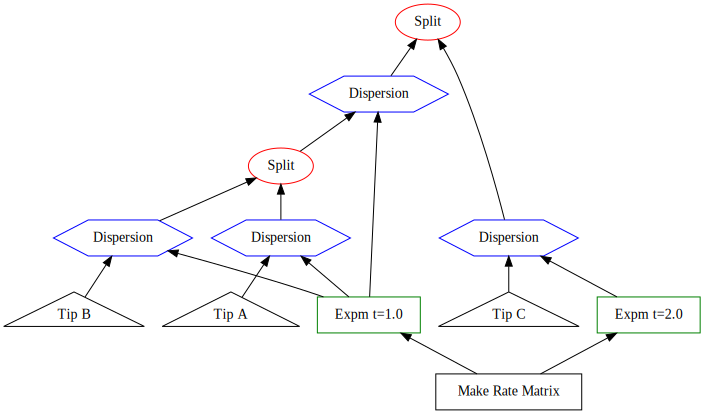
\includegraphics[width=\linewidth]{figures/full-operations.pdf}
  \caption{Tree in Figure~\ref{fig:ultra} decomposed into the operations used to compute the likelihood.}
  \label{fig:full-operations}
\end{figure}

\section{Comparing Distributions on Trees}

When comparing the results of Lagrange-ng and Lagrange, it can be difficult to know whether or not the results are
"close enough" to be the same. By way of example, scientific software will typically, instead of asking if two numbers
are exactly equal to one another, ask if they are closer than some small number called $\epsilon$. This is due to the
limitations in the IEEE 754 format, which is how real numbers are encoded in nearly all modern computers. A more
complete explanation of this phenomenon is outside the scope of this paper, and is extensively discussed in any textbook
on numerical computing, but for our purposes it is sufficient to say that differences in the order of operations will
generally yield different results, even when the results should algebraically equal.

Lagrange-ng does not escape this this limitation of the IEEE 754 standard. So, in order to fairly compare results, we
must take this into account. One can examine, by eye, each distribution individually and compare the distributions by
hand, but this is time consuming and error prone. Therefore, it is desirable to construct a metric between distributions
on trees in order to automatically compare the results.

Consider an example, where we have two sets of ancestral range distributions computed by differing methods using the
same tree. Let us call those distributions $d_1$ and $d_2$. The distribution for node $n$ is then represented by the
notation $d_i(n)$. Since the tree shared between the two distributions, we can match the node level distributions in a
one-to-one mapping between the two sets of distributions. We will index the individual elements of the distribution
either by the list of regions names or the binary notation for regions. For instance, if we have a distribution over
regions $A, B,$ and $C$, then an entry of distribution for node $n$ might be indexed as $d_1(n, AB)$. Equivalently, we
can use a binary notation to write $d_1(n, 110)$.

In this example, the first thought would be to treat $d_1(n)$ and $d_2(n)$ as vectors, and simply compute the cosine
distance between distributions. This will indeed produce a metric, but it has some undesirable qualities to it. For
example, suppose we have a distribution over 5 regions: $A, B, C, D$, and $E$ where $d_1(n, AB) = 1.0$. If we use the
cosine distance to compute the distance between $d_1(n)$ and $d_2(n)$ where $d_2(n, ABC) = 1.0$, then the resulting
distance will be 1.0, as the vectors are orthogonal. However, this is the same distance as if instead $d_2(n, CDE) =
  1.0$ as it is also orthogonal to $d_1(n)$. But, there is a very real sense in which the prediction $AB$ is much closer
to $ABC$ than $CDE$. In the first case, the predicted ranges differ by only one region, whereas in the second case, the
predicted ranges differ by \textit{every} region.

Since the cosine distance doesn't account for the available transitions between states in the DEC model, we should pick
a distance that is aware. To do this, we first embed the two distributions into a hypercube graph. A hypercube is graph
with $2^n$ nodes and each node is connected to $n$ other nodes (see Figure~\ref{fig:hypercube} for an example).
Importantly, the edges of a hypercube graph correspond to the valid transitions between states in the DEC
model\footnotemark.

\footnotetext{Some readers might have noticed in Figure~\ref{fig:hypercube} that the edges don't distinguish a direction
  of the edges, which means that transitions \textit{out} of the extinct state are valid. While conceptually this is a
  problem, for the purposes of computing a distance, it will not affect the results, as taking the path through the
  extinction state is equivalent to taking any other path of equal distance, of which there necessarily be due to the
  nature of the hypercube.}

Once the distributions are embedded in a hypercube graph, we can compute the distance between each distribution as the
``amount of effort required to turn one distribution into the other''. This is the Wasserstein metric, also known as the
Earthmover's distance, and is what we base our distance off of. Suppose we have the distributions $D1$ and $D2$ from
Figure~\ref{fig:distributions-example}. In order to turn $D1$ into $D2$, we need to find a way to move $0.25$ ``earth''
from node \texttt{10} to node \texttt{01}. Two example solution can be seen in Figure~\ref{fig:earthmovers-example}.
While the distance computation in Figure~\ref{fig:earthmovers-example} is straightforward, in general finding the
minimum distance requires the use of an optimization routine.

To find the minimum distance, we elected to express the problem as a linear programming problem. Specifically, we solve

\begin{align}
               & \min_x \textstyle \sum_i x_i \nonumber \\
  \text{such } & \text{that } Ax = b                    \\
               & x_i \geq 0 \nonumber
\end{align}

Where $A$ is the constraint matrix induced by the hypercube, and $b = d_1(n) - d_2(n)$ I.E. difference between the two
distributions. If we have a distribution with $s$ states then we can produce $A$ by creating $s-1$ rows and $s(2^{s}-1)$
columns. The rows represent the nodes of the graph, and the columns represent the edges of the graph, split in two for
each direction of flow. The entries of $A$ are defined as:
\begin{equation}
  A(n, e) = \begin{cases}
    1  & \text{If } e \text{ points to } n        \\
    -1 & \text{If } e \text{ points away from } n \\
    0  & \text{Otherwise.}
  \end{cases}
\end{equation}
Please note that there are only $n-1$ rows. This is because the final row will just be expressible as a linear
combination of the previous rows, and so will add no constraints to the problem. Additionally, we choose to suppress
edges leading away from the extinct state, to be consistent with the model. By suppressing these edges, we remove $s$
columns from the matrix as well.

As an example, the distance between the distributions in Figure~\ref{fig:distributions-example} can be computed with the
matrix
\begin{equation*}
  A = \begin{pmatrix}
    1  & 0  & 1  & 0  & 0 & 0 \\
    -1 & -1 & 0  & 0  & 1 & 0 \\
    0  & 0  & -1 & -1 & 0 & 1 \\
  \end{pmatrix}
\end{equation*}
and the vector
\begin{equation*}
  b = \begin{pmatrix}
    0    \\
    0.25 \\
    0.25 \\
  \end{pmatrix}.
\end{equation*}

Finally, in order to normalize the distance, we divide the result by maximum possible path length, which happens to be
the number of \textit{regions}.

\begin{figure}
  \begin{center}
    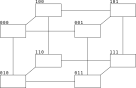
\includegraphics[width=0.95\textwidth]{figures/hypercube-distribution.pdf}
  \end{center}
  \caption{An example 3 dimensional hypercube with associated region names in binary notation.}
  \label{fig:hypercube}
\end{figure}

\begin{figure}
  \begin{center}
    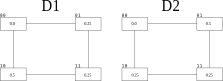
\includegraphics[width=0.95\textwidth]{figures/example-distributions.pdf}
  \end{center}
  \caption{Two example distributions, displayed as 2d-hypercubes (squares).}
  \label{fig:distributions-example}
\end{figure}

\begin{figure}
  \begin{center}
    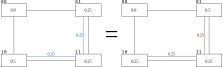
\includegraphics[width=0.95\textwidth]{figures/example-earthmovers.pdf}
  \end{center}
  \caption{Distributions from Figure~\ref{fig:distributions-example} with the Wasserstein metric applied. On the left,
    we choose to move $0.25$ units of ``mass'' from node \texttt{10} to node \texttt{01}. This requires 2 transitions,
    shown in blue, for a total of $0.5$ distance. On the right, we choose to transfer mass from node \texttt{01} to node
    \texttt{10}, which yields the same result.}
  \label{fig:earthmovers-example}
\end{figure}


\section{Experiments}
\label{sec:experiments}

\subsection{Investigating the Optimal Threading Configuration}

Because Lagrange-ng implements both course and fine grained parallelization, we need to investigate the optimal
threading configuration for a given dataset. To this end, we generated datasets with 50 or 100 taxa and 5, 6, 7, or 8
regions. This yielded a total of 8 dataset configurations. In addition to the dataset configurations, we also generated
the 6 threading configurations with a total number of 32 threads. For each of these dataset and threading
configurations, we ran 100 trials and recorded the times. The results from these runs can be seen in
Figure~\ref{fig:threading-configurations}.

\begin{figure}
  \begin{center}
    \includegraphics[width=0.95\textwidth]{figures/threading_violin.png}
  \end{center}
  \caption{Plot of the threading configurations on various dataset sizes. 100 datasets were generated for each Taxa,
    Region, and Threading Configuration parameters. Each dataset was generated randomly, similar to how datasets are
    constructed in the rest of this work.}
  \label{fig:threading-configurations}
\end{figure}

\subsection{Determining the parallel efficiency of Lagrange-ng}

Given the results from the previous experiment to determine the optimal threading configuration, we choose to determine
the parallel efficiency of the Lagrange-ng using only workers. This is to say, we only increased the number of threads
allocated to the coarse grained tasks. To this end we tested Lagrange-ng with 1, 4, 8, 16, and 32 threads by generating
100 datasets for each threading configuration. We did this with datasets with 6 regions and 100 and 500 taxa. We
computed the mean of the execution times for the runs with a single thread, and used this value to compute the
realized speedups.

\begin{figure}
  \begin{center}
    \includegraphics[width=0.95\textwidth]{figures/peff_100_taxa.png}
  \end{center}
  \caption{Parallel efficiency plot for a datasets with 100 taxa and 6 regions. Please notice the log-log scaling. The
    actual values plotted are 3.0, 4.1, 4.7, 4.8 for 4, 8, 16, 32 threads, respectively. The ratio of the realized
    speedup to the optimal speedup is 0.742873, 0.513696, 0.295814, 0.149044 for 4, 8, 16 and 32 threads respectively.}
  \label{fig:peff-100-taxa}
\end{figure}

\begin{figure}
  \begin{center}
    \includegraphics[width=0.95\textwidth]{figures/peff_500_taxa.png}
  \end{center}
  \caption{Parallel efficiency plot for a datasets with 500 taxa and 6 regions. Please notice the log-log scaling. The
    actual values plotted are 3.3, 5.5, 7., 9.3 for 4, 8, 16, and 32 threads, respectively. The ratio of the realized
    speedup to the optimal speedup is 0.83, 0.69, 0.49, 0.29 for 4, 8, 16, and 32 threads, respectively.}
  \label{fig:peff-100-taxa}
\end{figure}


\section{Discussion}
\label{sec:discussion}

Regarding the optimal threading configuration, Figure~\ref{fig:threading-configurations} shows that allocating all the
threads to workers is normally optimal. Occasionally, allocating 2 threads per worker is slightly faster. This is
slightly surprising, and might indicate that the linear algebra library used has issues with lock contention. If this is
the case, then changing the library might improve results. However, there are still sequential parts of the likelihood
computation which does not benefit from the fine grained parallelization, so this will have improvement a limit.

The threading efficiency of Lagrange-ng's coarse grained parallelization ranges between  0.74 and 0.14. This is
expected, as the method of parallelization is based on the tree topology. Children nodes must be evaluated before parent
nodes can be evaluated, which leads to a dependencies which prevent perfect parallel efficiency from being achieved.
This means that, for every likelihood evaluation, there is a period where there is less work available than threads. In
this case the threads idle, and do no meaningful work. However, we expect that as the number of taxa grows, the
efficiency of this method should increase, as the proportion of time spent in this "work starved" period is lower.
Results from the threading configuration experiments suggest that this can efficiency can be improved further on some
datasets by allocating 2 threads per worker.

\bibliographystyle{acm}
\bibliography{references}

\end{document}
